\part{Entrega 0}

\section{Comandos Para Correr Arquitectura X86 en Arquitectura ARM}

Debido a que trabajo en MAC, la arquitectura utilizadas es ARM 64, donde el requerimiento para las librerias es X86, por lo que se debe correr una instancia de X86 en la arquitectura ARM, donde para activar el entorno, se utilizan los siguientes comandos:

Primero se llama la instancia en una arquitectura X86

\begin{verbatim}
    arch -x86_64 python3 -m venv x86_env
\end{verbatim}

Luego se activa

\begin{verbatim}
    source x86_env/bin/activate
\end{verbatim}

Para instalar las librerias necesarias

\begin{verbatim}
    arch -x86_64 pip install <librerias>
\end{verbatim}

Finalmente debo correr el codigo desde la instancia

\begin{verbatim}
    arch -x86_64 python3 <ruta> .py
\end{verbatim}


    


\section{Calculos Manuales}

El codigo realizado para calcular el reticulado se encuentra en el \href{https://github.com/LukasWolff2002/PROYECTO_3_MCOC/blob/main/CODIGO/CODIGO_MANUAL/solucion_reticulado.py}{siguiente link}, donde, para calcular la seccion de las barras, se utilizo el \href{https://github.com/LukasWolff2002/PROYECTO_3_MCOC/blob/main/CODIGO/CODIGO_MANUAL/tipo_barras.py}{siguiente codigo}.

\begin{table}[H]
    \centering
    \begin{tabular}{|c|c|c|c|c|}
    \hline
    \textbf{Barra} & \textbf{Esfuerzo Interno} & \textbf{D$_{int}$, D$_{ext}$ [mm]} & \textbf{Tensiones Internas} & \textbf{Fuerza Critica Pandeo} \\ 
    \hline
    AB & 89.411 & (10, 28.500) & 159.835 & 508.521 \\ 
    AL & 15.000 & (10, 20.000) & 63.662 & 100.932 \\ 
    LK & 0.000 & (10, 20.000) & 0.000 & 227.096 \\ 
    LB & 0.000 & (10, 20.000) & 0.000 & 176.805 \\ 
    BC & 71.874 & (10, 26.000) & 158.876 & 541.368 \\ 
    BK & 30.000 & (10, 20.000) & 127.324 & 798.385 \\ 
    KJ & 0.000 & (10, 20.000) & 0.000 & 227.096 \\ 
    JC & 30.000 & (10, 20.000) & 127.324 & 204386.560 \\ 
    JI & 0.000 & (10, 20.000) & 0.000 & 227.096 \\ 
    CI & 64.321 & (10, 25.000) & 155.994 & 575.617 \\ 
    IH & 0.000 & (10, 20.000) & 0.000 & 403.727 \\ 
    IE & 70.062 & (10, 26.000) & 154.871 & 1012.850 \\ 
    HE & 30.000 & (10, 20.000) & 127.324 & 2150.023 \\ 
    HG & 0.000 & (10, 20.000) & 0.000 & 403.727 \\ 
    GE & 0.000 & (10, 20.000) & 0.000 & 339.901 \\ 
    GF & 15.000 & (10, 20.000) & 63.662 & 227.096 \\ 
    EF & 86.488 & (10, 28.000) & 160.993 & 899.137 \\ 
    \hline
    \end{tabular}
    \caption{Informacion Barras}
\end{table}

\textbf{Nota:} todas las barras se encuentran en esfuerzo de comprecion.

\begin{table}[H]
\centering
\begin{tabular}{|c|c|c|}
\hline
\textbf{Key} & \textbf{FS Fluencia} & \textbf{FS Pandeo} \\ 
\hline
AB & 1.314 & 5.687 \\ 
AL & 3.299 & 6.729 \\ 
BC & 1.322 & 7.532 \\ 
BK & 1.649 & 26.613 \\ 
CI & 1.346 & 8.949 \\ 
IE & 1.356 & 14.456 \\ 
EF & 1.304 & 10.396 \\ 
\hline
\end{tabular}
\caption{Factor de Seguridad Fluencia y Pandeo}
\end{table}

\textbf{Nota:} solo se consideran las barras que tienen algun esfuerzo interno significante para el calculo del FS.


\subsection{Calculo de Deformacion}



\section{Opensees}

EL codigo utilizado para hacer el modelo en Opensees se encuentra en el \href{https://github.com/LukasWolff2002/PROYECTO_3_MCOC/blob/main/CODIGO/OPENSEES/E0_Wolff.py}{siguiente link}, donde los esfuerzos obtenidos son los siguientes:

\begin{table}[H]
    \centering
    \caption{Esfuerzos internos en las barras (fuerzas axiales)}
    \label{tab:esfuerzos_internos}
    \begin{tabular}{|c|c|}
        \hline
        \textbf{Barra} & \textbf{Fuerza Axial (KN)} \\
        \hline
        AL & 15.03 \\
        AB & 89.39 \\
        LB & 0.06  \\
        LK & 0.05  \\
        KB & 30.03 \\
        BC & 71.82 \\
        KJ & 0.79  \\
        KC & 0.74  \\
        JC & 30.00 \\
        CD & 63.53 \\
        JI & 0.79  \\
        IH & 0.00  \\
        IE & 70.06 \\
        HE & 30.00 \\
        EF & 0.00  \\
        HG & 0.00  \\
        EF & 86.49 \\
        GF & 15.00 \\ \hline
    \end{tabular}
\end{table}

\textbf{Nota:} Se observa claramente una relacion directa con los resultados manuales, donde la pequeña variacion nace de la adicion de la barra \textbf{KC}.

\subsection{Deformaciones}

Para el calculo de las deformaciones, se asume una seccion igual para todas las barras, donde, segun los datosa calculados manualmente, la seccion nesesaria es (10,28.5), los resultados obtenidos son los siguientes:

\begin{figure}[H]
    \centering
    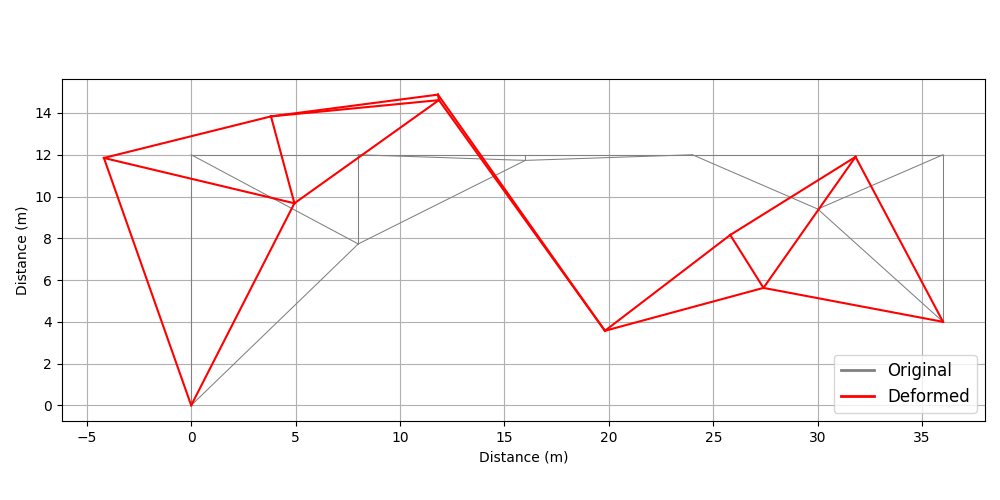
\includegraphics[width=0.8\textwidth]{GRAFICOS/deformed_truss.png}
    \caption{Deformaciones en los nodos}
    \label{fig:deformaciones}
\end{figure}

La deformacion observada en el nodo D/I es:

\begin{equation}
    \delta_x = -0.041897044917005404 \quad \delta_y =  -0.08428973931863179
\end{equation}




